%%%%%%%%%%%%%%%%%%%%%%%%%%%%%%%%%%%%%%%%%%%%%%%%%%%%
% Pre-requisite: Define your model name in the preamble
% \newcommand{\ModelName}{DLCM} 
%%%%%%%%%%%%%%%%%%%%%%%%%%%%%%%%%%%%%%%%%%%%%%%%%%%%

\section{Data}
To ensure experimental reproducibility, we build our corpus entirely from open-source data and tokenize it using the DeepSeek-v3 \cite{liu2024deepseek} tokenizer. Our corpus spans multiple domains, including web text (English and Chinese), mathematics, and code, forming a comprehensive foundation for core language understanding across linguistic, factual, and reasoning abilities.

The composition of our pretraining data is intentionally designed to serve two critical objectives. First, it balances breadth and specialization: web text provides broad natural language coverage, while mathematics and code enhance structured reasoning. Second, and more importantly for our architecture, this diversity is essential for learning robust dynamic segmentation. By exposing the model to domains with drastically different information densities (e.g., highly structured code syntax vs. verbose natural language prose), we force the learned boundary predictor to discover content-adaptive segmentation strategies that generalize across diverse tasks. English and Chinese web text are weighted more heavily to ensure multilingual alignment, while specialized datasets like MegaMath-Web and OpenCoder-Pretrain are included to fine-tune the model's handling of high-entropy transitions.

To demonstrate the architectural benefits of \ModelName{} rather than gains from data curation, we do not apply aggressive filtering; instead, we use data whose quality aligns with standard open-source corpora. \Cref{tab:training_data_details} summarizes the statistics.

\begin{table}[ht]
\centering
\small
\caption{\textbf{Statistics of the pretraining data.}}
\label{tab:training_data_details}
\begin{tabular}{l|cc}
\toprule
\textbf{Data Source} & \textbf{Ratio} & \textbf{Tokens (B)} \\
\hline
Nemotron-CC \cite{su2024nemotron} (English Web) & 50\% & 500 \\
MAP-CC \cite{du2024chinese} (Chinese Web) & 25\% & 250 \\
OpenCoder-Pretrain \cite{Huang2024OpenCoderTO} & 15\% & 150 \\
MegaMath-Web \cite{zhou2025megamath} & 10\% & 100 \\
\hline
\textbf{Total} & \textbf{100\%} & \textbf{1,000} \\
\bottomrule
\end{tabular}
\end{table}


\section{Scaling Laws for \ModelName{}}

To determine the optimal architecture and hyperparameters for \ModelName{}, we conduct a comprehensive exploration using scaling laws. We first introduce a decoupled optimization strategy to handle the heterogeneous nature of our architecture, followed by the mathematical formulation of our scaling objectives.

\subsection{Decoupled $\mu$P for Heterogeneous Architectures}

\subsubsection{Formulation of $\mu$P}

To ensure consistent feature learning dynamics across varying scales and compression rates, we adopt the Maximal Update Parametrization ($\mu$P). Unlike standard transformers with uniform width, our architecture requires decoupled scaling for the token-level components ($\mathcal{E}, \mathcal{D}$) with width $d_{\text{token}}$ and the concept-level backbone ($\mathcal{M}$) with width $d_{\text{concept}}$.

We define distinct width multipliers relative to a base width $d_{\text{base}}$:
\begin{equation}
    s_{\text{token}} = \frac{d_{\text{token}}}{d_{\text{base}}}, \quad s_{\text{concept}} = \frac{d_{\text{concept}}}{d_{\text{base}}}
\end{equation}

Following standard $\mu$P practice, we adjust initialization variances and optimization hyperparameters separately for each component group:

\begin{itemize}
    \item \textbf{Initialization:} All hidden linear weights $W \in \mathbb{R}^{d_{\text{out}} \times d_{\text{in}}}$ are initialized with variance $\sigma_{\text{base}}^2 \cdot s^{-1}$, where $s \in \{s_{\text{token}}, s_{\text{concept}}\}$ corresponds to the layer's width. Embedding weights use fixed $\sigma_{\text{base}}^2$.
    
    \item \textbf{Learning Rates:} To stabilize feature learning, hidden layer learning rates are scaled inversely to width:
    \begin{align}
        \eta_{\mathcal{E}, \mathcal{D}} &= \eta^{\text{base}}_{\text{token}} \cdot s_{\text{token}}^{-1} \\
        \eta_{\mathcal{M}} &= \eta^{\text{base}}_{\text{concept}} \cdot s_{\text{concept}}^{-1}
    \end{align}
    Biases and embedding weights retain the fixed learning rate $\eta^{\text{base}}_{\text{others}}$.

    \item \textbf{Output Scaling:} To ensure the logits remain $O(1)$ effectively, the final decoder projection $W_{\text{unemb}}$ is scaled during the forward pass:
    \begin{equation}
        \text{logits} = \frac{1}{s_{\text{token}}} \cdot (\mathbf{h}_{\text{final}} W_{\text{unemb}}^\top)
    \end{equation}

    \item \textbf{Optimizer Stability:} The AdamW $\epsilon$ parameter for each layer is scaled by $s^{-1}$, matching the respective component width.
\end{itemize}

\subsubsection{Hyperparameter Tuning and Verification}
\begin{figure}[t]
    \centering
    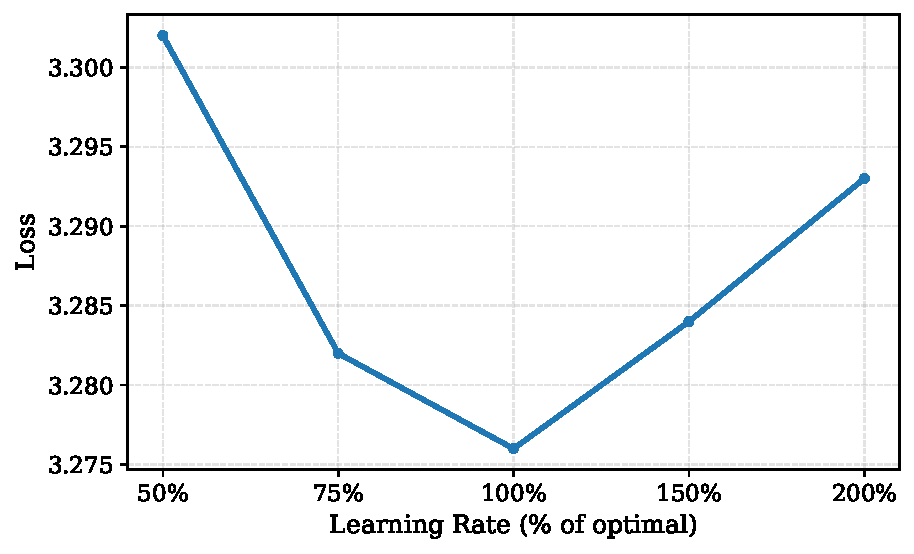
\includegraphics[width=0.47\textwidth]{sweep_concept.pdf}
    \hfill
    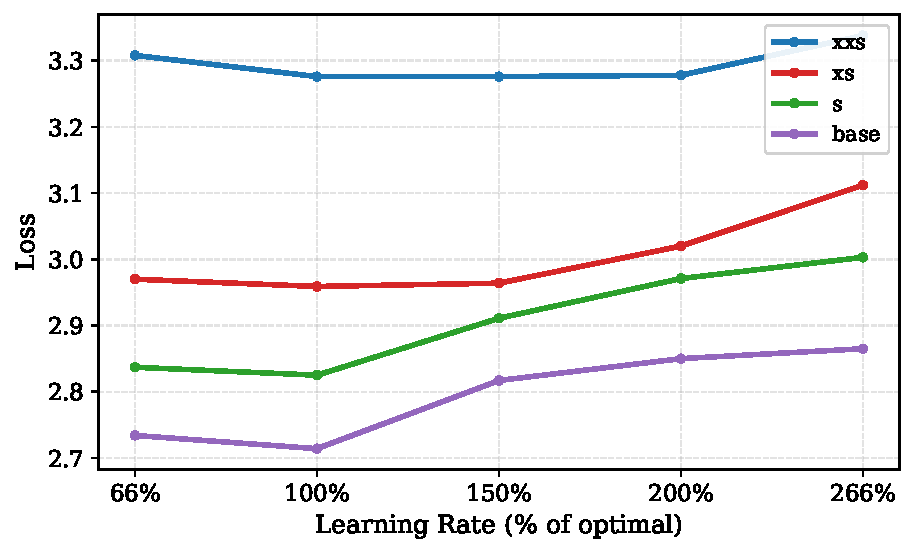
\includegraphics[width=0.47\textwidth]{sweep_both_concept_encoder_decoder_v2.pdf}
    \caption{
    \textbf{Hyperparameter tuning and transfer under $\mu$P.}
    \textbf{Left:} We sweep $\eta^{\text{base}}_{\text{concept}}$ while fixing $\eta^{\text{base}}_{\text{token}}$ at its $\mu$P-predicted value on the 87M proxy model. The loss curve shows a well-defined minimum near $100\%$.
    \textbf{Right:} We jointly scale both base learning rates by the same factor and observe consistent minima across model sizes (87M–834M), validating the zero-shot transferability of $\mu$P-derived hyperparameters.
    }
    \label{mup_exp}
\end{figure}


Following the protocol proposed by \citet{yang2022tensor}, we adopted a two-stage strategy: tuning hyperparameters on a small proxy model and verifying their transferability on larger scales.

\paragraph{Proxy Model Tuning.} We performed coordinate descent on the base learning rates using a proxy model with 87M parameters. For each hyperparameter group, we iteratively swept over a multiplicative grid of $\{0.5, 0.75, 1.5, 2.0\}$ relative to the current best value until the validation loss stabilized. Empirically, we observed that the optimal base learning rates for the token and concept components were approximately equal ($\eta^{\text{base}}_{\text{concept}} \approx \eta^{\text{base}}_{\text{token}}$). We show the result of tuning $\eta^{\text{base}}_{\text{concept}}$ while keeping $\eta^{\text{base}}_{\text{token}}$ in Figure~\ref{mup_exp}, which means the actual learning rates depend on the ratio of the widths between the token and concept components in this unequal-width model. This consistency suggests that the explicit width-dependent scaling factors defined previously successfully account for the structural differences between components, stabilizing the effective learning rates across different widths.

\paragraph{Transfer Verification.} To validate the zero-shot hyperparameter transfer, we trained larger models (274M, 468M, 834M parameters) using the optimal $\eta^{\text{base}}$ values derived from the 87M proxy. Then we perturbed the predicted learning rates by simultaneously scaling $\eta^{\text{base}}_{\text{token}}$ and $\eta^{\text{base}}_{\text{concept}}$. As shown in Figure~\ref{mup_exp}, deviating from the $\mu$P-predicted learning rates resulted in degraded performance, confirming that the optimal hyperparameters found on the proxy model transfer effectively to larger scales without further tuning. Overall, this confirms that $\mu$P effectively stabilizes training for our unequal-width architecture, provided that the learning rates for the token and concept components are decoupled and scaled inversely to their respective widths. This finding extends standard scaling laws to heterogeneous designs, ensuring consistent optimality across scales.

\subsection{Scaling Law Formulation}

\subsubsection{Experimental Setup}
To validate our scaling hypotheses, we constructed a grid of models by varying the concept-layer parameter ratio $P \in \{30\%, 50\%, 70\%\}$ and the compression ratio $R \in \{2, 4, 8\}$. Models were trained on a budget of $200$B tokens, resulting in three primary model scales for analysis: \textbf{Small} (274M), \textbf{Medium} (468M), and \textbf{Large} (833M). All scaling exponents ($\delta_1, \delta_2, \gamma$) are \emph{shared globally} across all model scales and compression ratios, and are fitted \emph{once} using the joint training trajectories.
Only scale-independent offset terms are allowed to vary across configurations.
This design constrains the degrees of freedom of the model and avoids post-hoc overfitting to individual scales.


\subsubsection{Mathematical Formulation}
We extend the Chinchilla scaling framework~\cite{hoffmann2022training} by introducing (i) compression-aware behaviour and (ii) architectural decomposition. The resulting loss law is:

\begin{equation}
\label{eq:scaling_law}
L(N, D, R, P) 
= E_0
+ \frac{A_{\text{token}}}
       {(N(1-P) + t_{\text{token}})^{\delta_1}}
+ \frac{A_{\text{concept}} \, R^{\gamma}}
       {(NP + t_{\text{concept}})^{\delta_2}}
+ \frac{A_{\text{data}}}
       {(D + t_{\text{data}})^{\alpha}}.
\end{equation}

where $N$ is total parameters, $D$ is dataset size, $R$ is compression ratio, $P$ is concept-layer parameter ratio, and $E_0$ is the irreducible loss floor. This formulation disentangles token-processing efficiency, concept-processing efficiency (controlled by exponent $\gamma$), and data scaling.

\subsubsection{Decay-Phase Power Law}
Since our training protocol involves Weight-Sharing-and-Decay (WSD), we explicitly model the late-stage regime. We fit a simplified decay law to the fractional loss reduction $\Delta_{\text{decay}}$ in the 90\%–99\% token window:
\begin{equation}
\Delta_{\text{decay}} = k \, L_{\text{stable}}^{\,a} R^{\,b} N^{\,c}
\end{equation}
Obtained via log-linear regression, this model achieves $R^2 = 0.93$, accurately predicting late-stage loss drops across all scales.

\begin{figure}[t]
  \centering
  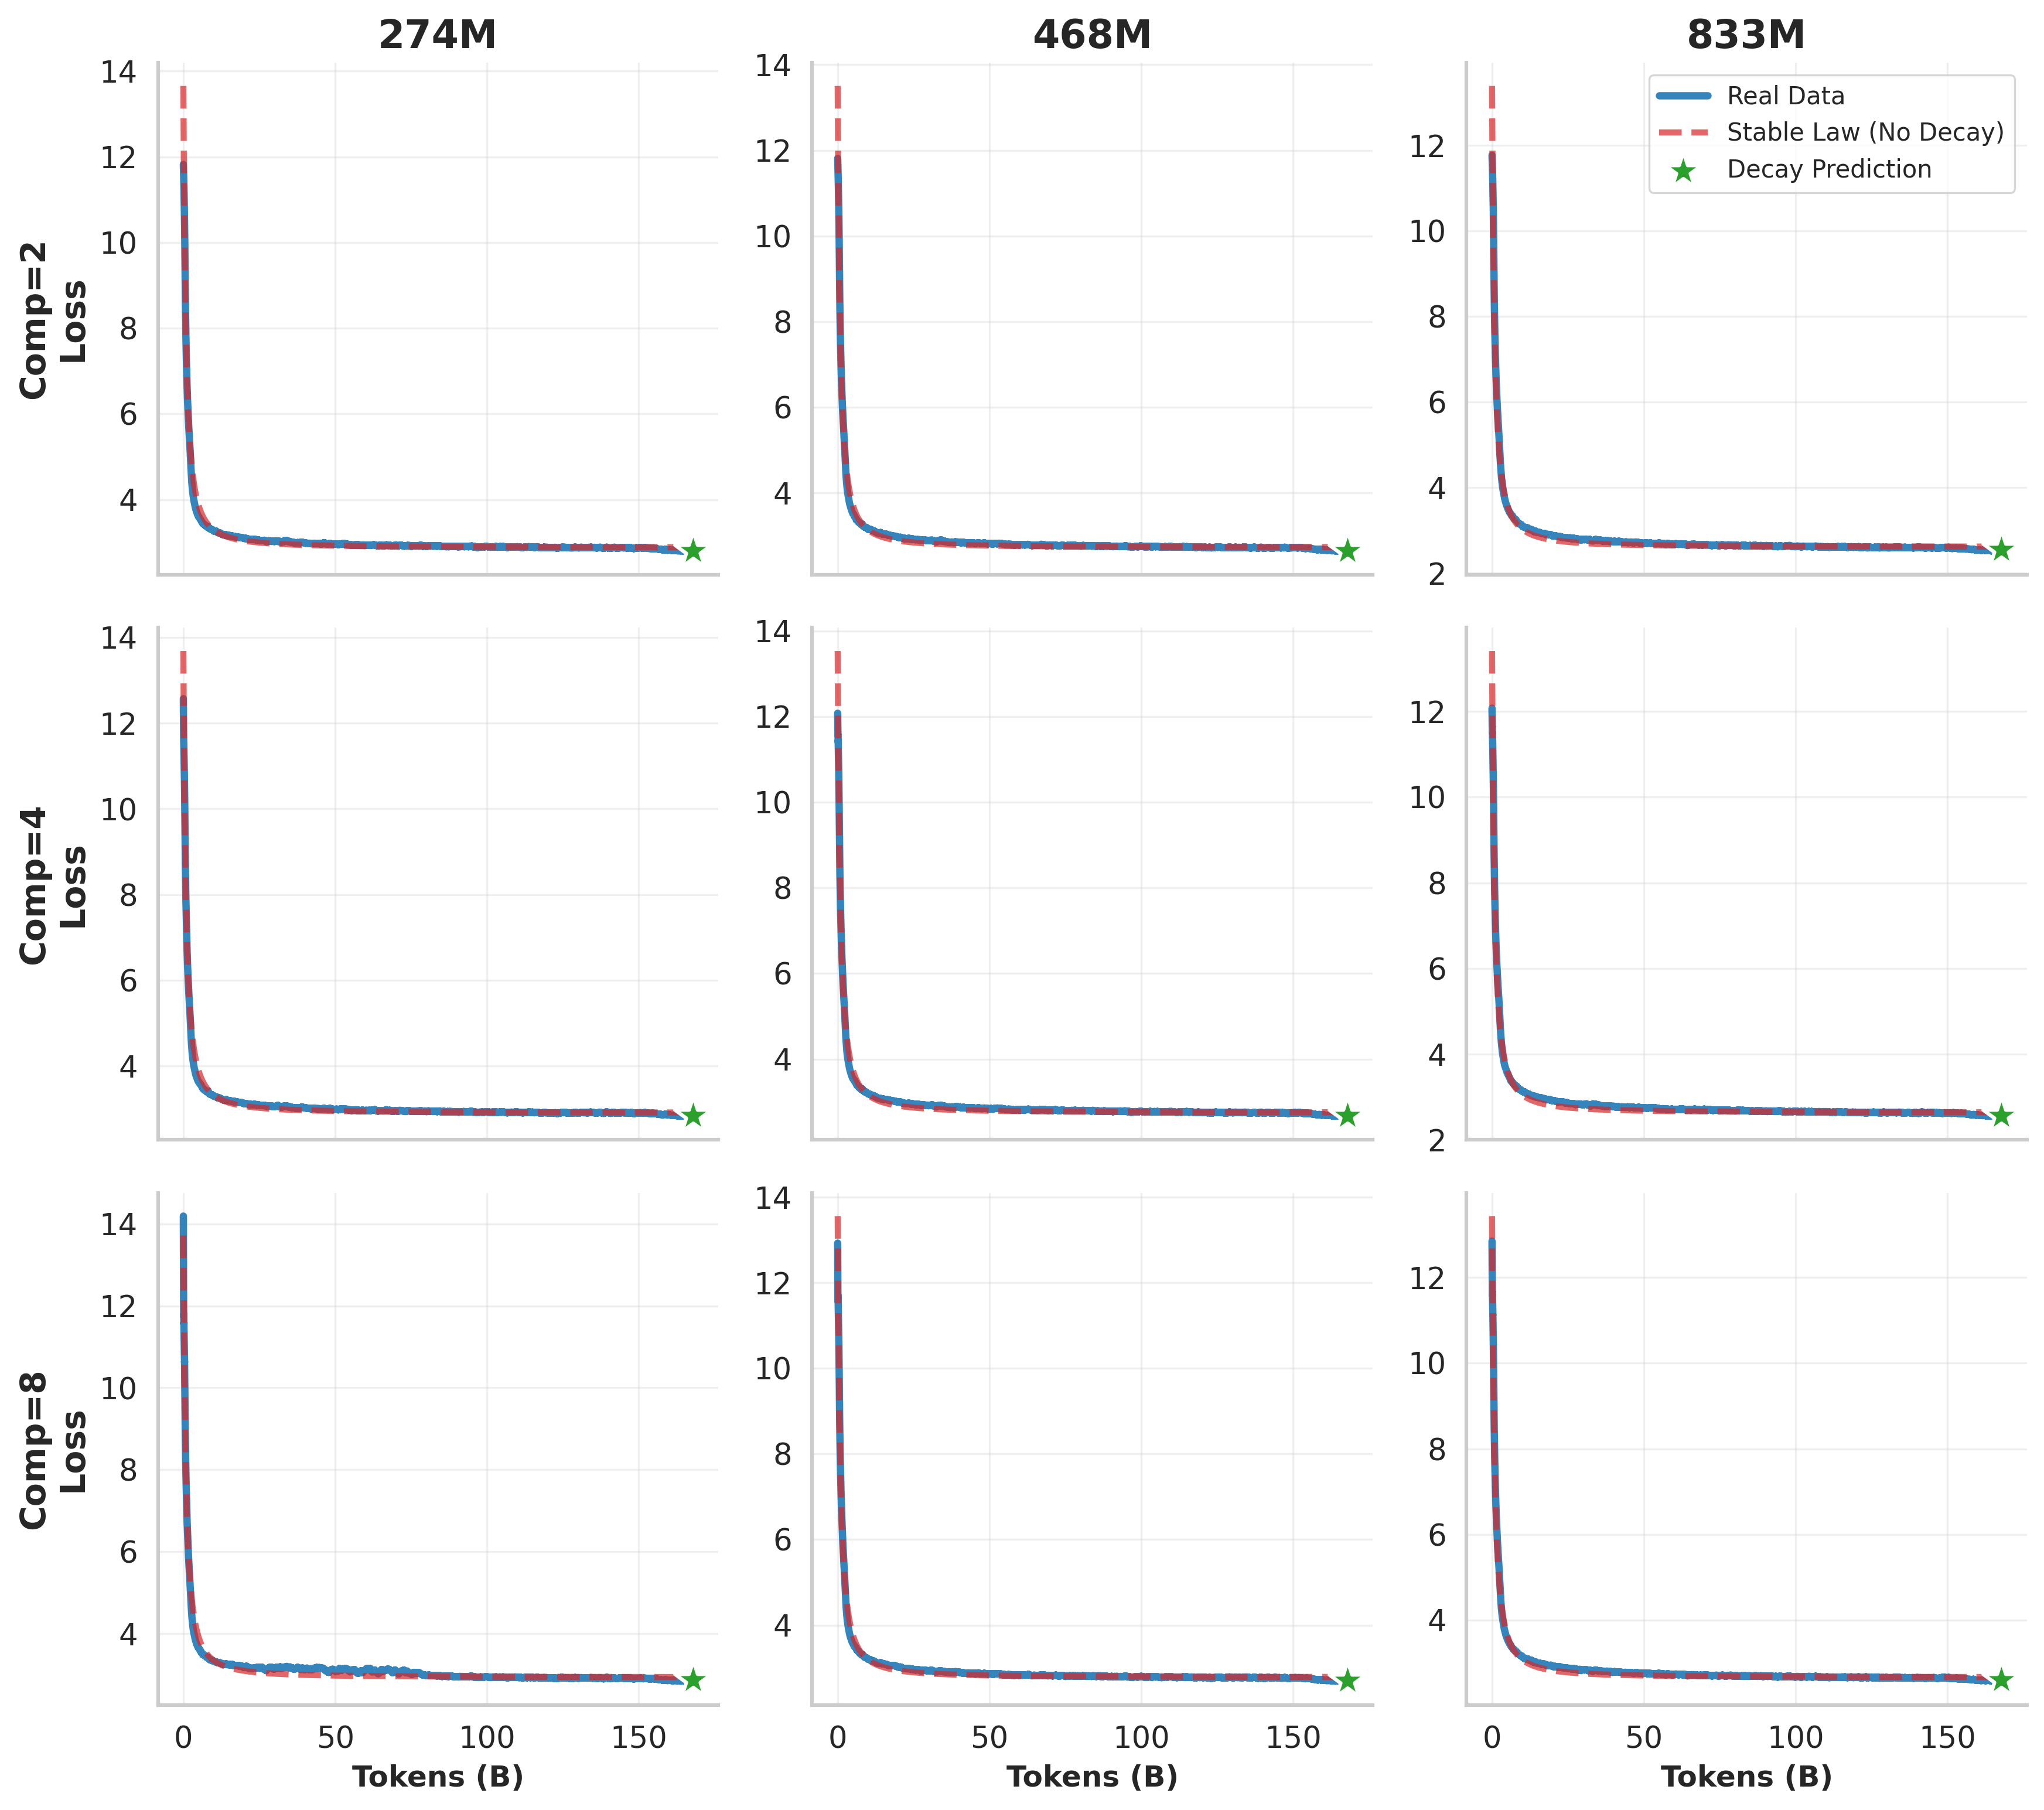
\includegraphics[width=0.9\linewidth]{full_training_linear.png}
  \caption{\textbf{Full training trajectory fit.} Comparison between predicted loss (Equation~\ref{eq:scaling_law}) and empirical loss across model sizes (274M--833M), compression factors $R \in \{2,4,8\}$, and training budgets. The joint fit achieves $R^2 > 0.98$.}
  \label{fig:full_training_fit}
\end{figure}

\begin{figure}[t]
  \centering
  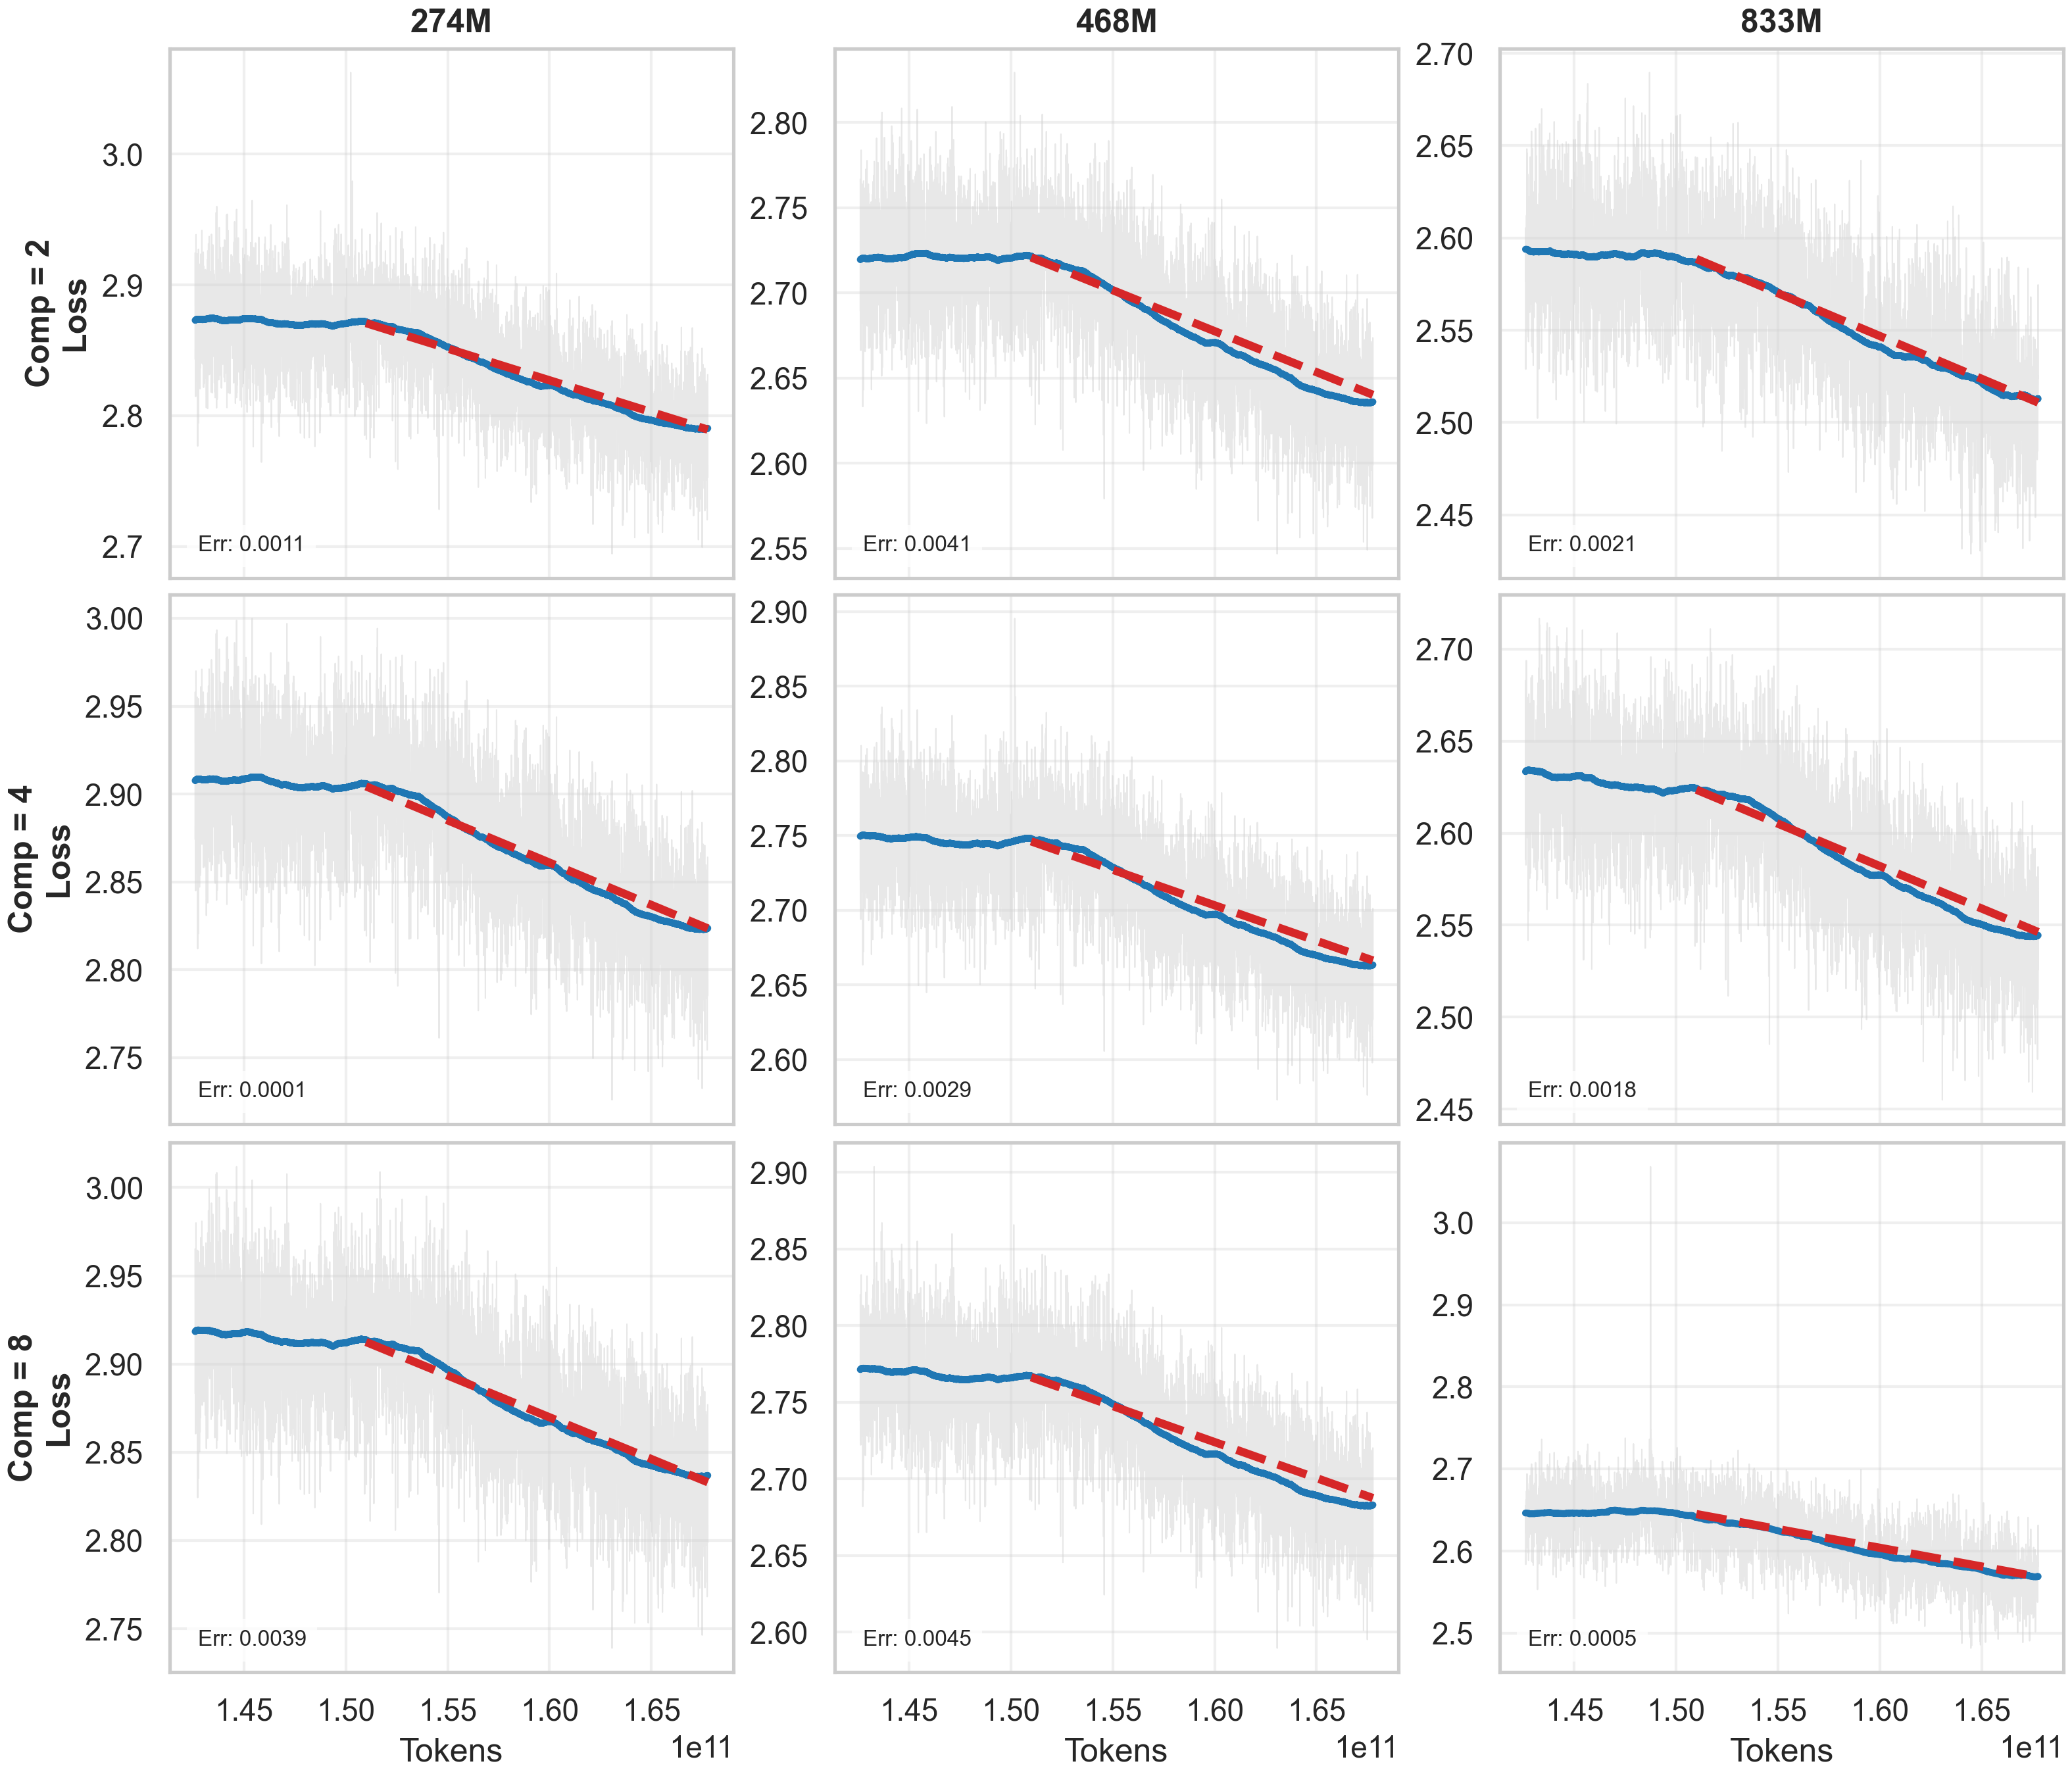
\includegraphics[width=0.9\linewidth]{robust_decay_fit.png}
  \caption{\textbf{Decay-phase fit.} Simplified fit on the final portion of training tokens, validating that our WSD scaling law accurately captures late-stage behaviour with $R^2 = 0.93$.}
  \label{fig:decay_fit}
\end{figure}

As shown in Figure~\ref{fig:full_training_fit} and Figure~\ref{fig:decay_fit}, our methodology—incorporating a tail-focused sampling strategy and weighting late-token regions—ensures the law generalizes reliably across both architectural and data scales.

\subsection{Optimal Configuration Analysis}

\subsubsection{Architectural Efficiency}
Figure~\ref{fig:wsd_scaling_law_fit}(a) illustrates the Loss/FLOPs efficiency across different backbone proportions $P$ and compression ratios $R$.

\begin{figure*}[t]
  \centering
  \begin{minipage}{0.48\linewidth}
    \centering
    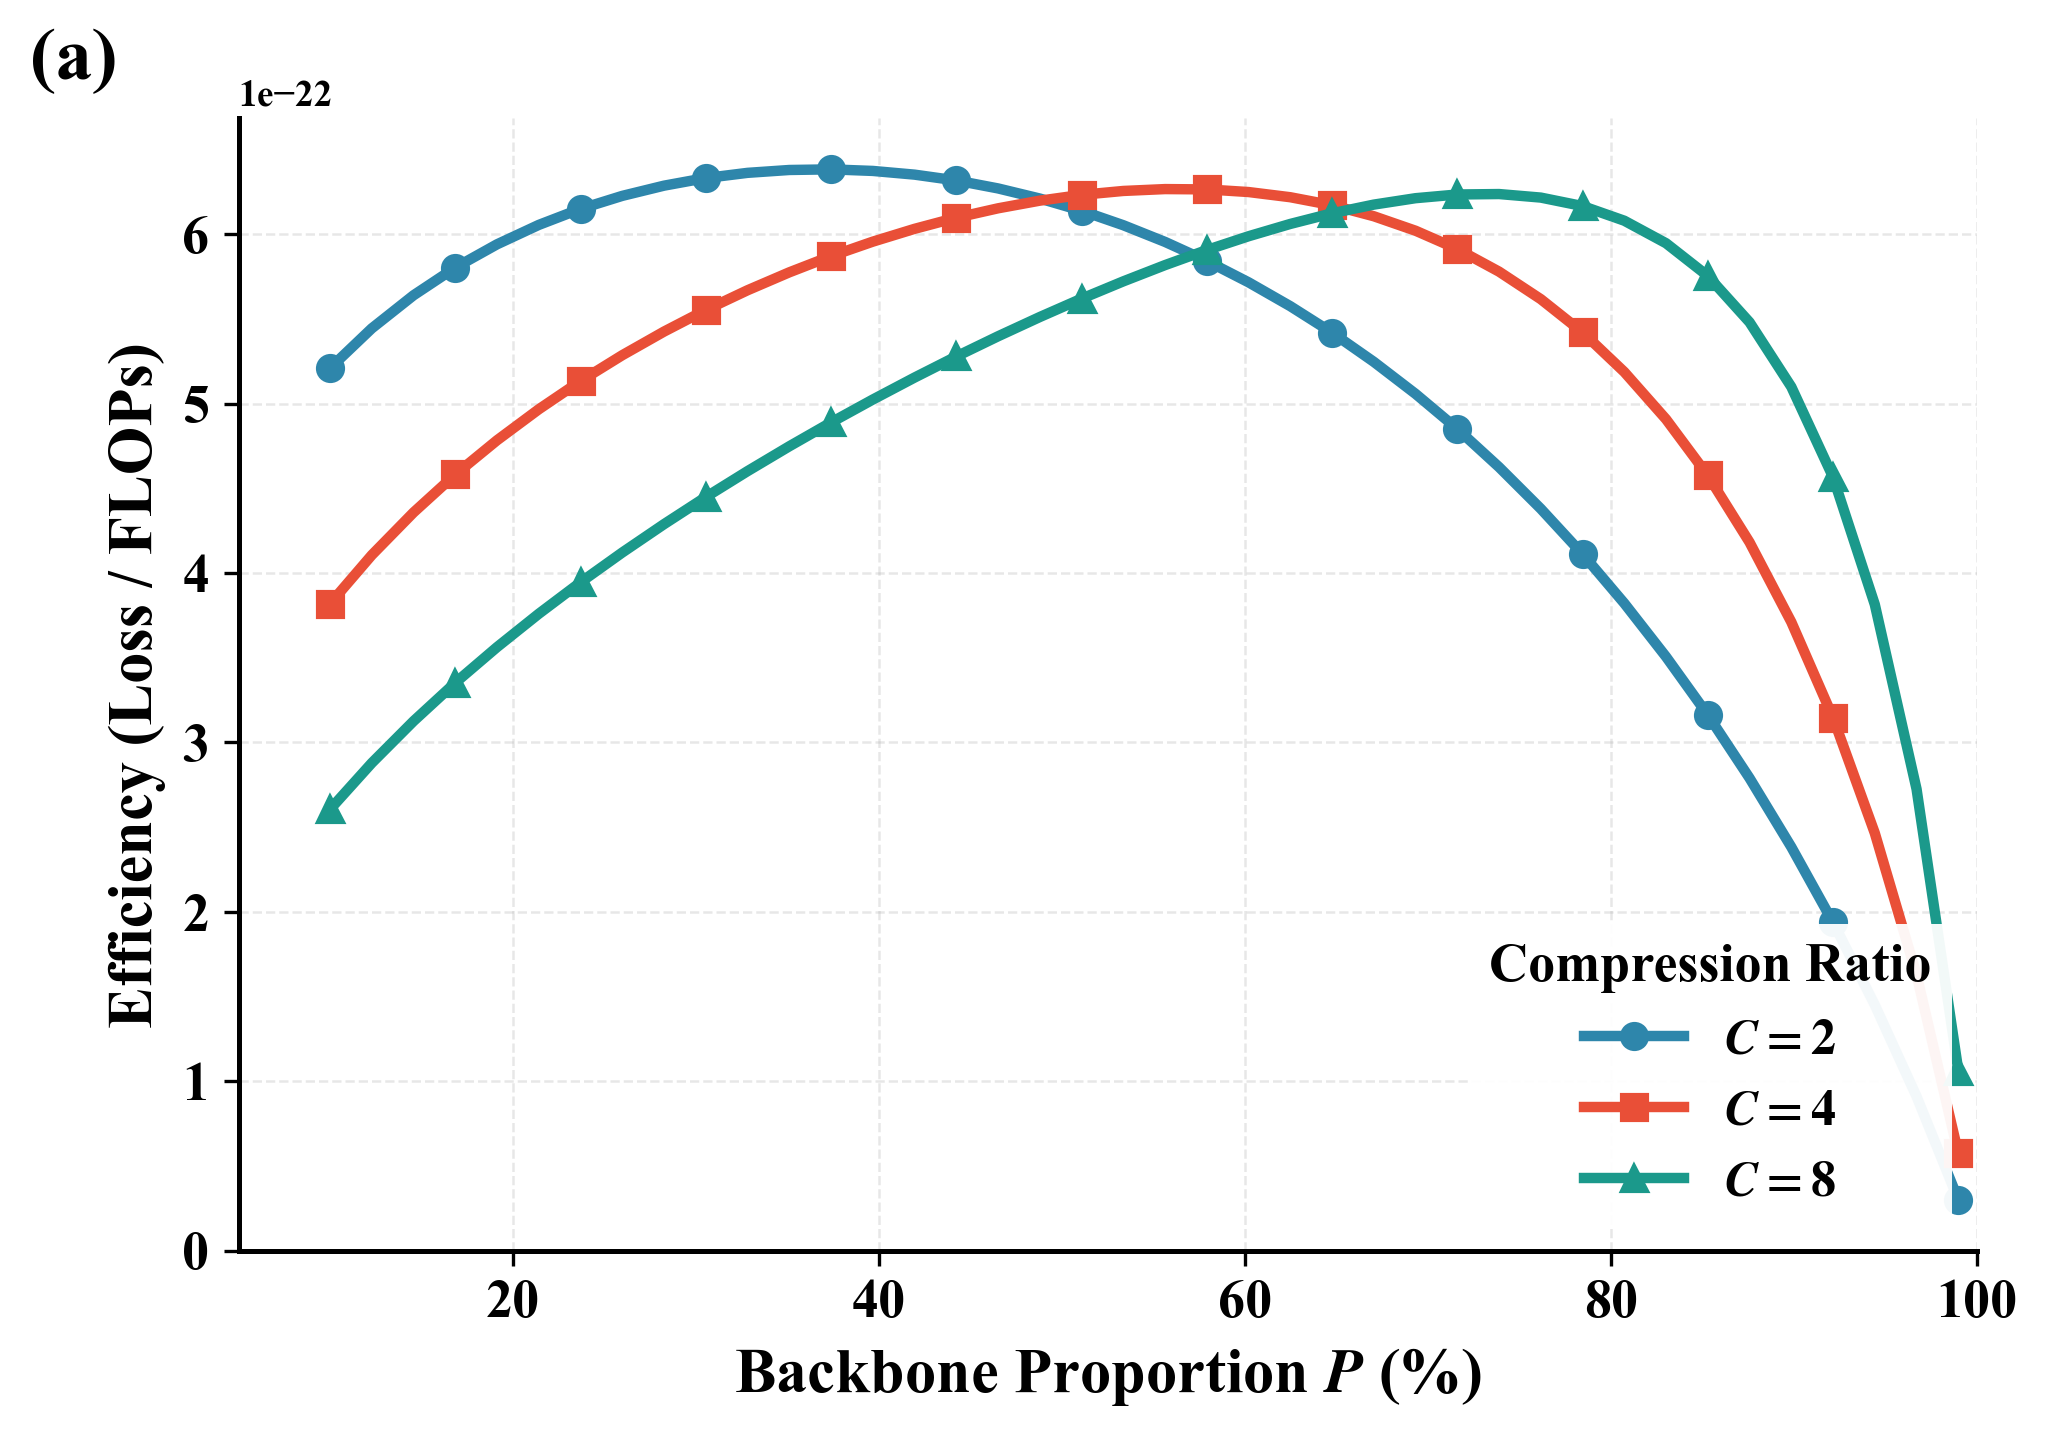
\includegraphics[width=\linewidth]{figure_efficiency.png}
  \end{minipage}\hfill
  \begin{minipage}{0.48\linewidth}
    \centering
    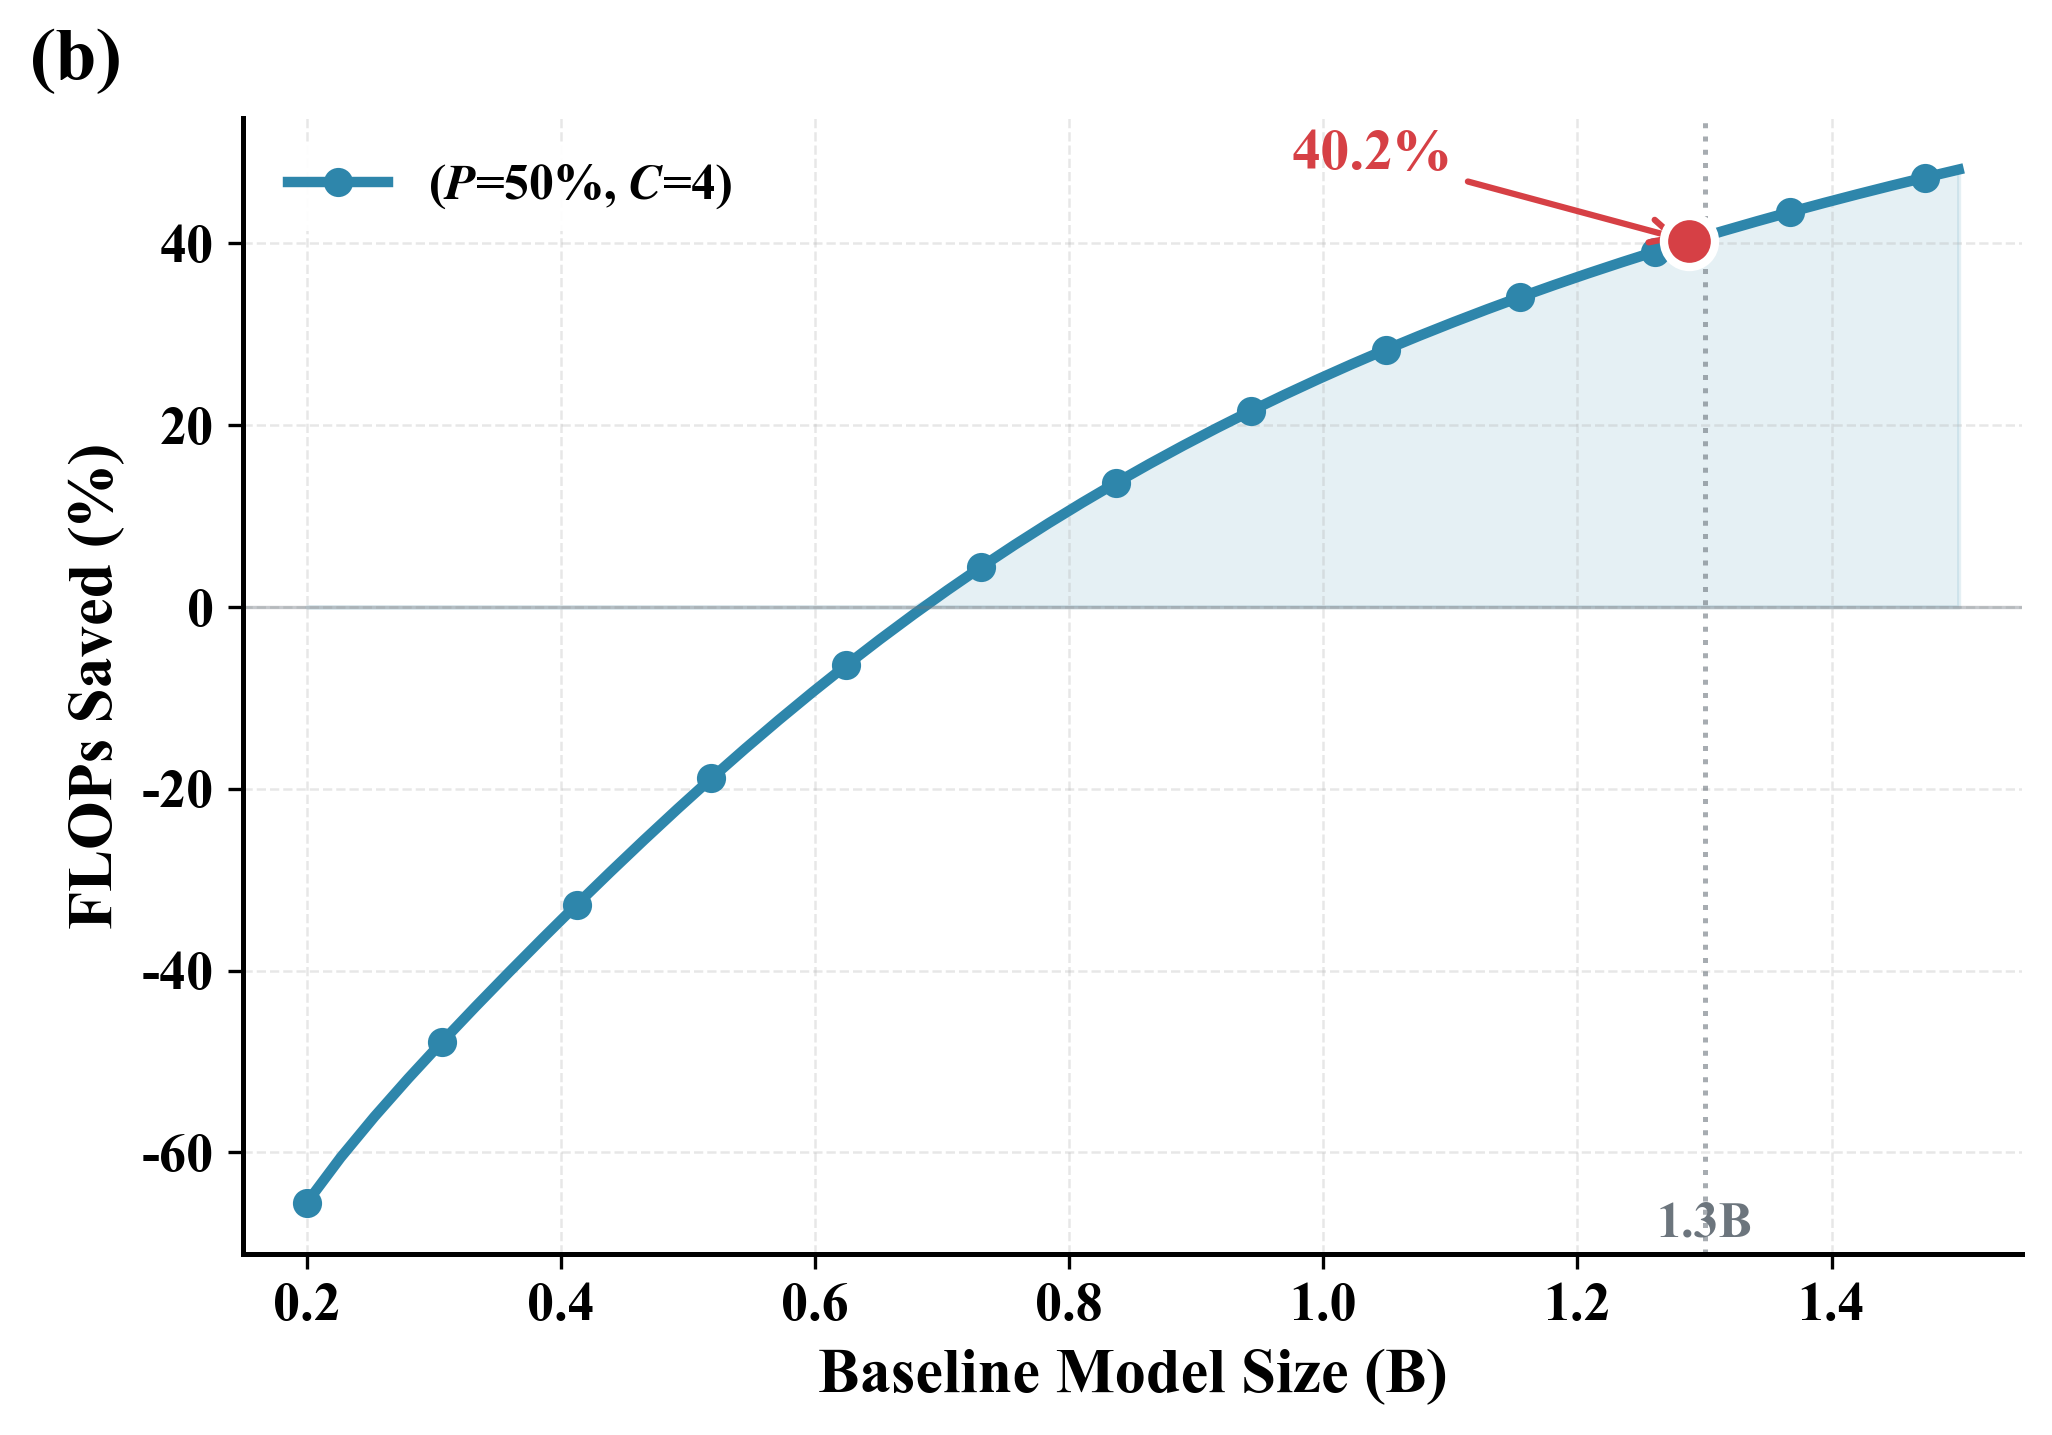
\includegraphics[width=\linewidth]{figure_flops_savings.png}
  \end{minipage}
  \caption{Efficiency analysis of the \ModelName{} architecture. 
(a) Architectural efficiency (Loss/FLOPs) across backbone proportions $P$ 
for different compression ratios $R$. (b) FLOPs savings compared to baseline 
models of varying sizes, with \ModelName{} configured at $P=60\%, R=4$.}
  \label{fig:wsd_scaling_law_fit}
\end{figure*}

\paragraph{Selection of Compression Ratio ($R=4$):}
While higher compression rates offer theoretical FLOPs savings, we empirically selected $R=4$ as the primary configuration. This decision is driven by the granularity of concept compression; as discussed in Appendix~\ref{appendix:segmentation}, a compression ratio of 4 aligns better with the intuitive semantic segmentation of tokens into concepts, offering the best balance between training stability and computational efficiency.

\subsection{Scaling Law Validation and Verification}

We developed a unified scaling-law estimator by jointly modeling the full-training loss trajectory and the late-stage decay behavior. To ensure robustness, we adopted a tail-focused sampling strategy that emphasizes curvature near convergence, performing fits on 100B-token trajectories while validating against 1T-token limits. As shown in Figure~\ref{fig:full_training_fit} and Figure~\ref{fig:decay_fit}, our estimator maintains a fitting error below 0.05 across the entire window. 

This high-fidelity fitting allows for a critical verification of our architectural properties: our scaling law yields an effective compute multiplier prediction of approximately \textbf{1.4}. This value aligns closely with the standard baseline factor of \textbf{1.34}. This consistency confirms that our theoretical projections are grounded in established empirical norms and that the architecture scales predictably under the proposed law.

% \subsection{MuP Validation}
% \xingweitodo{here for shaowen }

\section{Experiments}

\subsection{Main Results}

We compare \ModelName{} against a parameter-matched baseline that
follows the LLaMA~\cite{touvron2023llama} architecture. Both models are
trained from scratch on our proprietary dataset, using the same global
batch size, learning rate, and sequence length as reported in the LLaMA
paper. Each model is trained on 1T tokens. Results on 12 standard
zero-shot benchmarks are summarized in
Table~\ref{tab:categorized_comparison_step238000}.


Our model follows an \emph{encoder--compressor--decoder} architecture with learned concept circulation, explicitly redistributing computation from uniform token-level processing to adaptive concept-level reasoning.
As a consequence, we do not expect uniform gains across all benchmarks.
Instead, performance differences directly reflect the architectural bias induced by semantic compression and boundary-aware compute allocation.

Overall, \ModelName{} achieves an average accuracy of \textbf{43.92\%}, surpassing the baseline score of 41.23\% by \textbf{+2.69\%}.
However, these gains are highly non-uniform across tasks, revealing a clear separation between reasoning-dominant benchmarks and those that rely on fine-grained token-level alignment.

\paragraph{Reasoning-Dominant Tasks.}
We observe consistent and often substantial improvements on benchmarks that emphasize multi-step reasoning, hypothesis selection, and implicit commonsense inference.
Notable gains are achieved on \textbf{CommonsenseQA (+1.64\%)}, \textbf{HellaSwag (+0.67\%)}, \textbf{OpenBookQA (+3.00\%)}, \textbf{PIQA (+2.42\%)}, and both \textbf{ARC Easy (+2.61\%)} and \textbf{ARC Challenge (+1.77\%)}.
These tasks are characterized by non-uniform information density, where prediction difficulty concentrates around semantic transitions rather than being evenly distributed across tokens.
By compressing locally predictable spans and allocating the majority of model capacity to a high-dimensional concept backbone, \ModelName{} focuses computation on structurally salient regions.
This behavior is consistent with our loss distribution analysis in Section~7.2, which shows systematic loss reduction near concept boundaries.

\paragraph{Granularity-Sensitive Text Understanding.}
In contrast, we observe mild regressions on \textbf{BoolQ (-1.47\%)} and \textbf{RACE (-0.72\%)}.
These benchmarks depend heavily on fine-grained sentence-level entailment, polarity resolution, and subtle lexical cues.
The encoder--compress--decode paradigm inevitably reduces token-level granularity within concept interiors, which can obscure micro-level distinctions required for such tasks.
Importantly, this degradation is localized rather than uniform: while boundary tokens are modeled more accurately, mid-concept positions may trade off fine-grained precision for improved global coherence.
This trade-off manifests as the U-shaped loss profile observed in our mechanistic analysis.

\paragraph{Knowledge and Multilingual Benchmarks.}
For encyclopedic knowledge evaluation, we observe mixed behavior.
While \textbf{C-Eval (+1.71\%)} benefits from adaptive segmentation enabled by the Global Parser, slight regressions appear on \textbf{MMLU (-0.30\%)} and \textbf{CMMLU (-0.24\%)}.
These datasets reward relatively uniform factual recall across tokens, leaving less opportunity for boundary-aware compute reallocation.
This result further supports our central claim: \ModelName{} is structurally optimized for reasoning under non-uniform information density, rather than uniform memorization-heavy retrieval.

\paragraph{Architecture and Parameter Efficiency.}
Although \ModelName{} contains nearly \textbf{2$\times$} the total parameters of the baseline model (2.3B vs.\ 1.3B), this increase is deliberately concentrated in the concept-level backbone ($d_{\text{concept}}=3072$).
Because this backbone operates on a sequence compressed by $4\times$, the effective FLOPs per inference step remain comparable to the smaller baseline.
This validates our core design principle: shifting computation from redundant token-level processing to dense concept-level reasoning enables substantially larger effective capacity without incurring proportional inference cost.

% huakai
% The evaluation tasks can be categorized as follows:
% General Knowledge and Commonsense Reasoning
% HellaSwag/CommonsenseQA/OpenBookQA/PIQA/ARC easy/ARC Challenge/WinoGrande

% Reading Comprehension
% BoolQ/RACE

% comprehensive benchmark
% c-eval/cmmlu/mmlu

% referring to LLaMA2(https://arxiv.org/abs/2307.09288)

\begin{table}[htbp]
\centering
\caption{\textbf{Performance Comparison: DLCM vs. Baseline.} Zero-shot accuracy (\%) categorized by task type. Improvements are shown in \textcolor{green}{green} and regressions in \textcolor{red}{red}.}
\label{tab:categorized_comparison_step238000}
\renewcommand{\arraystretch}{1.2}
\setlength{\tabcolsep}{10pt}
\begin{tabular}{lccc}
\toprule
\rowcolor{gray!15}
\textbf{Task / Category} & \textbf{DLCM (Ours)} & \textbf{Baseline} & \textbf{Diff.} \\
\midrule
\multicolumn{4}{l}{\textit{Multi-choice General Knowledge / Common Sense}} \\

Commonsense QA  & \textbf{21.38} & 19.74 & \textcolor{green}{+1.64} \\
HellaSwag       & \textbf{46.66} & 45.99 & \textcolor{green}{+0.67} \\
Winogrande      & \textbf{57.22} & 56.20 & \textcolor{green}{+1.02} \\
OpenBookQA      & \textbf{26.80} & 23.80 & \textcolor{green}{+3.00} \\
PIQA            & \textbf{75.52} & 73.10 & \textcolor{green}{+2.42} \\
ARC Challenge   & \textbf{34.81} & 33.04 & \textcolor{green}{+1.77} \\
ARC Easy        & \textbf{69.91} & 67.30 & \textcolor{green}{+2.61} \\
MMLU            & 25.40 & \textbf{25.70} & \textcolor{red}{-0.30} \\
\midrule
\multicolumn{4}{l}{\textit{Multi-choice Text Understanding}} \\
BoolQ           & 62.54 & \textbf{64.01} & \textcolor{red}{-1.47} \\
RACE            & 35.31 & \textbf{36.03} & \textcolor{red}{-0.72} \\
\midrule
\multicolumn{4}{l}{\textit{Culture / Multilingual Knowledge}} \\
C-Eval          & \textbf{26.08} & 24.37 & \textcolor{green}{+1.71} \\
CMMLU           & 25.23 & \textbf{25.47} & \textcolor{red}{-0.24} \\
\midrule
\rowcolor{gray!15}
\textbf{Average} & \textbf{43.92} & 41.23 & \textcolor{green}{\textbf{+2.69}} \\
\bottomrule
\end{tabular}
\end{table}

% 优化后的 Table 3：合并为单一大表，消除中间空隙，强制对齐
\begin{table}[ht]
\centering
\caption{\textbf{Architecture Configuration Details.} A unified view of the parameter settings for Baseline (LLaMA-1.3B) and \ModelName{} (2.3B). Values are presented as \textit{Baseline / Ours}.}
\label{tab:architecture_comparison}
\small
\renewcommand{\arraystretch}{1.2} % 增加行间距，让表格更透气
\setlength{\tabcolsep}{5pt}       % 微调列间距

\begin{tabular}{ll @{\hspace{1.2cm}} ll} % @{\hspace{1.2cm}} 控制左右两部分中间的间距
    \toprule
    % --- 第一组表头 ---
    \multicolumn{2}{l}{\textbf{General Settings}} & \multicolumn{2}{l}{\textbf{Dimension Settings}} \\
    \cmidrule(r){1-2} \cmidrule(l){3-4} % 局部横线，中间断开，增加美感
    \textit{Metric} & \textit{Value} & \textit{Metric} & \textit{Value} \\
    \midrule
    Model Type      & Trans. / \textbf{DLCM}    & Hidden Size ($d_{\text{token}}$)   & 1,536 \\
    Total Params    & 1.3B / \textbf{2.3B}      & Main Hidden ($d_{\text{concept}}$) & -- / \textbf{3,072} \\
    Vocab Size      & 128,815                   & Interm. Size (Self)                & 4,096 / 6,144 \\
    Max Pos Emb     & 8k /8k         & Interm. Size (Cross)               & -- / 6,144 \\
    Activation      & Swish                     &                                    & \\ % 右边空一行，保持对齐
    \midrule
    
    % --- 第二组表头 ---
    \multicolumn{2}{l}{\textbf{Layer Configuration}} & \multicolumn{2}{l}{\textbf{Attention Configuration}} \\
    \cmidrule(r){1-2} \cmidrule(l){3-4}
    Total Layers    & 32                        & Attn Heads      & 24 / 24 \\
    Encoder Layers  & -- / \textbf{10}          & Backbone Heads  & -- / \textbf{48} \\
    Backbone Layers & -- / \textbf{16}          & KV Heads        & 24 / 12 \\
    Decoder Layers  & -- / \textbf{6}           & Backbone KV     & -- / \textbf{24} \\
    \bottomrule
\end{tabular}
\end{table}

\subsection{Analysis: Compute Allocation in Concept-Based Models}

\subsubsection{Experimental Setup}
To isolate the impact of concept-based compression on model behavior, we conduct a controlled comparison between our proposed concept model and a standard Transformer baseline. Both models utilize the same backbone architecture (1.3B parameters) and were trained on an identical subset of $100$B tokens from our pretraining corpus. This ensures that any observed differences in loss distribution are attributable solely to the compression mechanism and architectural changes, rather than discrepancies in training data or compute budget.

\subsubsection{Loss Distribution Analysis}
To understand how the model allocates computational resources, we evaluate the loss distribution across relative positions within concepts. We randomly selected 600 samples from the validation set and aligned the token-level losses based on their position within a segmented concept (e.g., the $i$-th token of a concept).

Figure~\ref{fig:loss_comparison} illustrates the average loss at the first 20 positions within each concept. The top panel compares raw loss values, while the bottom panel visualizes the differential: $\Delta L = L_{\text{concept}} - L_{\text{baseline}}$. Here, \textbf{green bars} ($\Delta L < 0$) indicate the concept model outperforms the baseline, while \textbf{red bars} ($\Delta L > 0$) indicate degradation.

\begin{figure}[h]
    \centering
    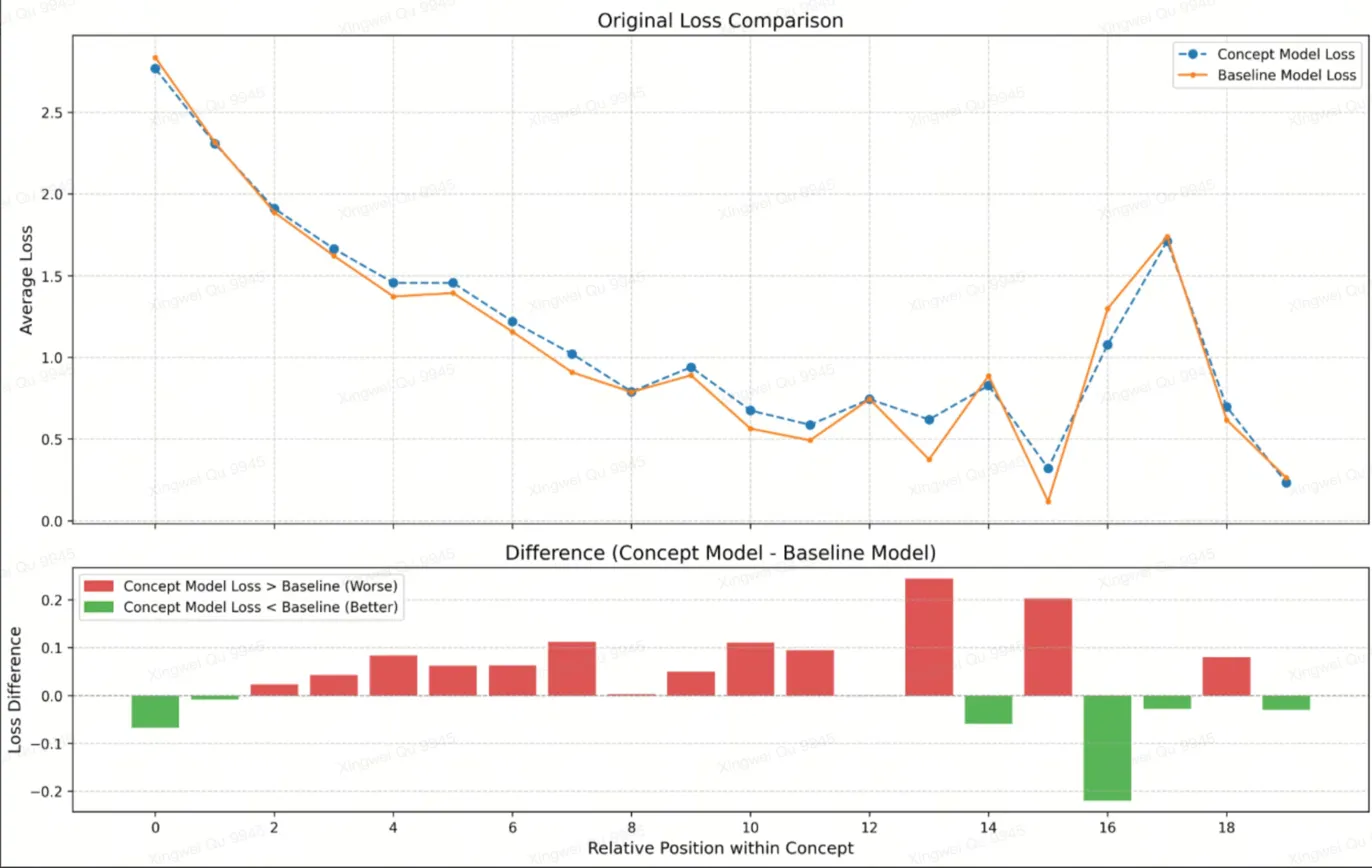
\includegraphics[width=0.8\textwidth]{budgets.png}
    \caption{Top: Average loss comparison between concept model (blue) and baseline model (orange) across relative positions within concepts. Bottom: Loss difference (Concept - Baseline), where \textbf{green indicates improvement} (lower loss) and red indicates degradation.}
    \label{fig:loss_comparison}
\end{figure}

The results reveal a distinct "U-shaped" improvement pattern that reflects the model's resource reallocation strategy:

\begin{enumerate}
    \item \textbf{Boundary Proficiency (Positions 0--2 \& 16+):} Consistent with the observation that concept models excel at initial and late positions (indicated by green bars), the architecture effectively captures the transition semantics. By explicitly modeling concept boundaries, the model reduces ambiguity at the start and end of semantic units, outperforming the baseline which treats these tokens uniformly.
    
    \item \textbf{Internal Complexity (Mid-positions):} In the middle of a concept (approx. positions 4--15), we observe a shift. While the baseline model often struggles here (higher absolute loss), the concept model's performance is mixed. The presence of red bars in certain mid-concept regions suggests that the compression mechanism forces the model to trade off some fine-grained token-level precision to maintain higher-level semantic coherence.
\end{enumerate}

This reallocation aligns with our hypothesis: the concept model sacrifices uniform token-level predictability (resulting in minor degradation at specific internal positions) to gain superior performance at semantic boundaries and structurally critical tokens. This strategic trade-off allows the model to "spend" its capacity on maintaining global coherence, explaining the downstream improvements despite non-uniform loss reduction.

\section{Ablation Studies}

\subsection{Analysis: End-to-End Discrete Boundary Learning vs. Decoupled Segmentation}

This experiment compares two boundary prediction mechanisms for sequence compression: a learned neural predictor with compression rate regularization (Section~\ref{sec:adaptive_compression}) and a rule-based predictor using cosine similarity. Starting with sequences of length $L=8192$, we track the average compressed length during training.

Figure \ref{fig:comparison} reveals starkly different behaviors. The \textbf{learned predictor (red)} exhibits severe instability: after initial compression to $\sim$2000 tokens, the compressed length steadily increases, eventually stabilizing at $\sim$4300 tokens ($1.9\times$ compression). This "creep-up" indicates the model progressively learns to compress less over time. In contrast, the \textbf{rule-based predictor (purple)} demonstrates exceptional stability, rapidly converging to $\sim$2000 tokens ($4\times$ compression) and maintaining this level consistently throughout training.

The learned predictor's instability stems from conflicting optimization objectives. Despite the compression rate regularization term $\mathcal{L}_{\text{aux}}$ designed to maintain the target compression ratio $R$, the primary cross-entropy (CE) loss creates much stronger gradients that penalize information loss and discourage compression:
\begin{equation}
\nabla_{\theta} \mathcal{L}_{\text{total}} = \underbrace{\nabla_{\theta} \mathcal{L}_{\text{CE}}}_{\text{anti-compression}} + \lambda \underbrace{\nabla_{\theta} \mathcal{L}_{\text{aux}}}_{\text{pro-compression}}
\end{equation}
Since $\|\nabla_{\theta} \mathcal{L}_{\text{CE}}\| \gg \lambda \|\nabla_{\theta} \mathcal{L}_{\text{aux}}\|$, the CE loss eventually dominates, forcing the predictor to reduce segmentation despite the regularization term.

The rule-based predictor avoids this conflict through a fixed decision rule: $p_t = \frac{1 - \cos(h_t, h_{t+1})}{2}$, with boundaries inserted when $p_t > \tau$. While the representations $h_t$ are learned, the segmentation rule itself is not optimized by the CE loss. This decoupling prevents the task loss from undermining the compression mechanism, ensuring stable and controllable compression ratios through the threshold parameter $\tau$.

\begin{figure}
    \centering
    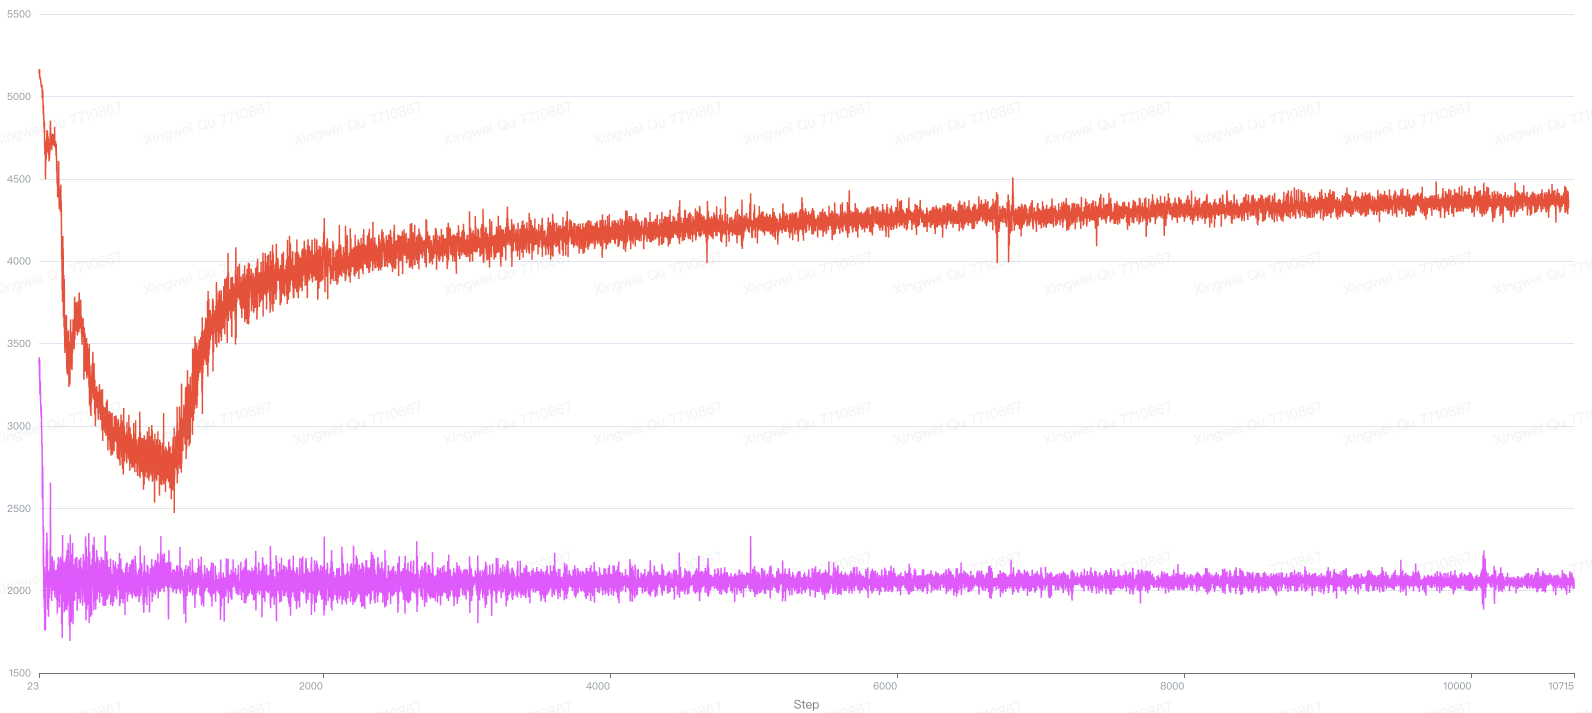
\includegraphics[width=0.8\textwidth]{red.png}
    \caption{Average compressed sequence length over training steps. \textbf{Red:} Learned Boundary Predictor. \textbf{Purple:} Rule-Based Predictor. The x-axis represents training steps, and the y-axis represents the average number of tokens post-compression.}
    \label{fig:comparison}
\end{figure}

\subsection{Global Regularization via Gradient Accumulation}

To further stabilize the learned boundary predictor, we investigate an alternative regularization strategy: computing the compression ratio loss over accumulated training examples rather than individual sequences (Section~\ref{sec:adaptive_compression}). This \textbf{global regularization} approach computes boundary statistics $F_{\text{global}}$ and $G_{\text{global}}$ across all tokens in $K$ micro-batches.

We train two 2.3B parameter models for 1T tokens with a target compression ratio of $R=2$: one with per-sequence regularization ("Normal") and one with global regularization ("Global Parser"). Table \ref{tab:ablation} presents the downstream performance and the actual realized compression ratios.

\begin{table}[htbp]
\centering
\caption{\textbf{Ablation Study: Global Parser vs. Normal.} Performance comparison on downstream tasks. Both models aim for a target compression ratio of $R=4$. The \textbf{Global Parser} achieves a realized ratio much closer to the target while consistently improving accuracy on most tasks.}
\label{tab:ablation}
\renewcommand{\arraystretch}{1.15} % 增加行高
\setlength{\tabcolsep}{10pt}       % 增加列间距

\begin{tabular}{lccc}
\toprule
\rowcolor{tabgray}
\textbf{Task} & \textbf{Global Parser} & \textbf{Normal} & \textbf{Metric} \\
\midrule
ARC Challenge   & \textbf{0.3038} & 0.2858 & Acc \\
ARC Easy        & \textbf{0.6296} & 0.6242 & Acc \\
Commonsense QA  & \textbf{0.2457} & 0.2228 & Acc \\
HellaSwag       & \textbf{0.3507} & 0.3499 & Acc \\
OpenBookQA      & 0.3220 & \textbf{0.3280} & Acc \\
PIQA            & \textbf{0.6806} & 0.6785 & Acc \\
\midrule
% 底部统计行，加背景色突出
\rowcolor{tabgray}
\textbf{Avg. Improvement} & \textcolor{green}{\textbf{+2.1\%}} & -- & -- \\
\textbf{Realized Ratio}   & \textbf{3.92} & 3.15 & (Target $R{=}4$) \\
\bottomrule
\end{tabular}
\end{table}

The global regularization approach achieves consistently better performance across most tasks (5 out of 6). Crucially, as shown in the bottom row of Table~\ref{tab:ablation}, the Global Parser maintains a realized compression ratio ($\sim$3.9) much closer to the target ($4.0$) compared to the Normal formulation, which tends to degrade towards lower compression.

The key insight is that enforcing a fixed compression ratio per sequence is overly restrictive. Real-world data exhibits varying information density. By relaxing the constraint to operate at the batch level, the global regularization allows the model to learn adaptive behavior—compressing repetitive code more aggressively while preserving dense technical text—effectively allocating the compression "budget" where it matters most.

\subsection{Content-Adaptive Compression Benefits}

To verify the adaptive behavior enabled by global regularization, we analyzed the segmentation granularity across different domains. Table~\ref{tab:compression_stats} presents empirical measurements of the average tokens per concept.

\begin{table}[h]
\centering
\begin{tabular}{lccc}
\hline
\textbf{Content Type} & \textbf{Target 8×} & \textbf{Target 4×} & \textbf{Target 2×} \\
\hline
Casual English    & 7.47 & 3.53 & 1.76 \\
Casual Chinese    & 8.38 & 4.36 & 1.76 \\
Technical English & 10.58 & 3.85 & 1.92 \\
Technical Chinese & 6.09 & 3.27 & 1.76 \\
Code              & 6.14 & 3.66 & 1.98 \\
Math/Science      & 7.42 & 4.41 & 1.91 \\
\hline
\end{tabular}
\caption{Average tokens per concept across content types and compression ratios. Values represent the actual granularity achieved for each target compression setting.}
\label{tab:compression_stats}
\end{table}

The data reveals significant variation in compression density across content types. For instance, at the 8× target, Technical English retains significantly more tokens per concept (10.58) compared to Technical Chinese (6.09) or Code (6.14). 

While the precise ranking of "optimal" length varies across compression targets (as noted in the fluctuation between content types), the \textbf{existence of this variation} is the critical finding. It confirms that the global regularization mechanism successfully decouples the compression objective from rigid per-sequence constraints. The model is not forcing a uniform segment length; instead, it adapts the granularity based on the inherent semantic density of the content. Code and structured text tend to be compressed into shorter, syntactic units, whereas dense prose is preserved in longer semantic chunks. This adaptivity—regardless of the specific order—allows the model to maximize information retention within the global compression budget.
\section{Conclusion}

We presented \textbf{Dynamic Large Concept Models (DLCM)}, a hierarchical language modeling framework that challenges the token-uniform computation paradigm underlying modern LLMs. By learning semantic boundaries from latent representations and shifting computation from tokens to variable-length concepts, DLCM enables reasoning to occur in a compact, semantically aligned space rather than repeatedly at the token level.

Beyond the architectural design, we showed that hierarchical compression necessitates new theoretical and optimization tools. We introduced a compression-aware scaling law that clarifies how compute should be allocated between token processing and concept-level reasoning under fixed FLOPs, and developed a decoupled $\mu$P parametrization that enables stable training and zero-shot hyperparameter transfer in heterogeneous architectures. Empirically, DLCM achieves consistent gains on reasoning-intensive benchmarks while reducing redundant computation, demonstrating a favorable accuracy--efficiency trade-off.

More broadly, our results suggest that scaling language models is not solely a matter of increasing parameters or data, but also of reconsidering \emph{where} computation is performed. We believe concept-level latent reasoning offers a promising direction for building more efficient and more reasoning-capable language models, and opens avenues for future work on adaptive abstraction, planning, and multi-level reasoning in large-scale neural systems.


\newpage
\section*{Contributions}

\textbf{Leading Authors}

Xingwei Qu, Shaowen Wang, Zihao Huang, Ge Zhang

\textbf{Leading Author Contributions}

Xingwei Qu: Conducts fundamental ablation studies and is responsible for the majority of the engineering implementation.

Shaowen Wang: Implements and advances the MuP (Maximal Update Parametrization) for hyperparameter tuning.

Zihao Huang: Implements noise based boundary prediction tricks.

Ge Zhang: Proposes the original idea and develops the demo prototype. Identifies and provides the key technique for the Global Parser.

\textbf{Core Contributors}

Kai Hua: Designs and constructs the training data entirely from open-source data.

Fan Yin: Contributes to the SGLang implementation and optimization.

Rui-Jie Zhu: Resolves bugs related to \ModelName{} and proposes the strategy of replacing the encoder with \ModelName{}.

Jundong Zhou \& Qiyang Min: Contributes to the project development and implementation.

\textbf{Other Contributors}

Zihao Wang, Yizhi Li, Tianyu Zhang, He Xing, Zheng Zhang, Yuxuan Song, Tianyu Zheng, Zhiyuan Zeng

\textbf{Corresponding Authors}

Chenghua Lin, Ge Zhang, Wenhao Huang